
\includegraphics[height=1.25cm]{images/pictograms/benchmark}

\includegraphics[height=1.25cm]{images/pictograms/tools}

\includegraphics[height=1.25cm]{images/pictograms/FEM}

%%%%%%%%%%%%%%%%%%%%%%%%%%%%%%%%%%%%%%%%%%%%%%%%%%%%%%%%%%%%%%%%%%%%%%%%%%%%%%%%%%%%%%%%%%%%%%%%%%%

\begin{flushright} {\tiny {\color{gray} python\_codes/fieldstone\_151/text.tex}} \end{flushright}

\lstinputlisting[language=bash,basicstyle=\small]{python_codes/fieldstone_151/keywords.key}

\par\noindent\rule{\textwidth}{0.4pt}

\begin{center}
\inpython
{\small Code: \url{https://github.com/cedrict/fieldstone/tree/master/python_codes/fieldstone_151}}
\end{center}

\par\noindent\rule{\textwidth}{0.4pt}

%%%%%%%%%%%%%%%%%%%%%%%%%%%%%%%%%%%%%%%%%%%%%%%%%%%%%%%%%%%%%%%%%%%%%%%%%%%%%%%%%%%%%%%%%%%%%%%%%%%

This \stone builds on \stone~\ref{f33} in the sense that in \stone~\ref{f33} 
free slip boundary conditions were implemented and tested on an annulus discretised 
by means of \QonePzero{} elements. We here implement and test the implementation 
of such boundary conditions on an annulus discretised by means of \QtwoQone{} elements.

One could envisage three ways to implemenent these boundary conditions:
\begin{itemize}
\item the rotating method (see Section~\ref{MMM-ss:fsbc_annulus}),
\item constraints applied to elemental matrix,
\item constraints via Lagrange multipliers
\end{itemize}

The code follows a standard approach when it comes to meshing, FEM, isoparametric
mapping, quadrature, solving, etc ...and the fluid is isothermal and incompressible.
Note that the code computes the strain rate tensor components by means of 3 different 
methods (it is based on \stone~\ref{f21}) but this is not relevant here.
Also the mesh exported to the vtu file is based on a subdivision of the elements into 
four bilinear quadrilaterals. In other words it means that 4 elements in paraview 
form a single 'real' element in the code.
By default all node are placed on concentric circles. However when the {\python trapezes}
integer variable is set to {\python 1} then all mid-edges nodes are then placed exactly 
in the middle of the corresponding corner nodes (obviously the middle node is then also 
moved to be at the center of the trapeze/element).
Free slip boundary conditions are only implemented at the surface ($r=R_2$).

\begin{center}
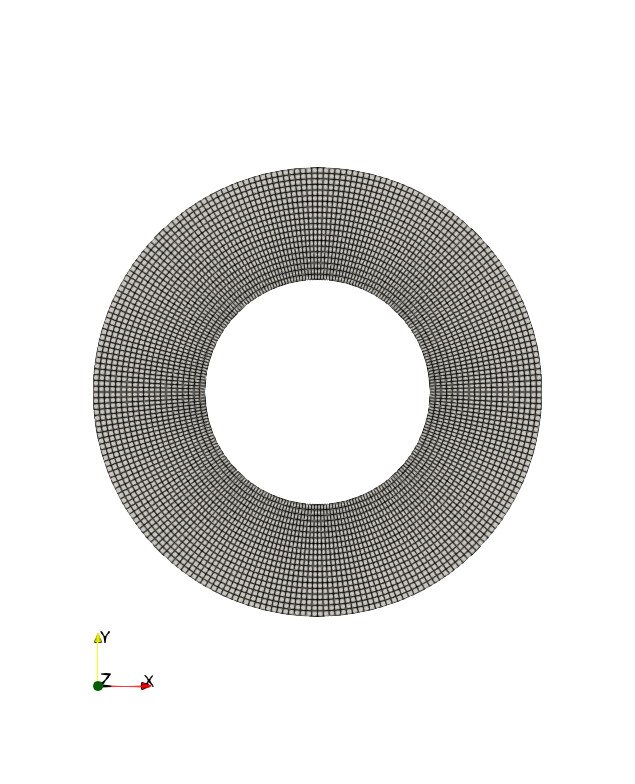
\includegraphics[width=5.6cm]{./python_codes/fieldstone_151/images/mesh}
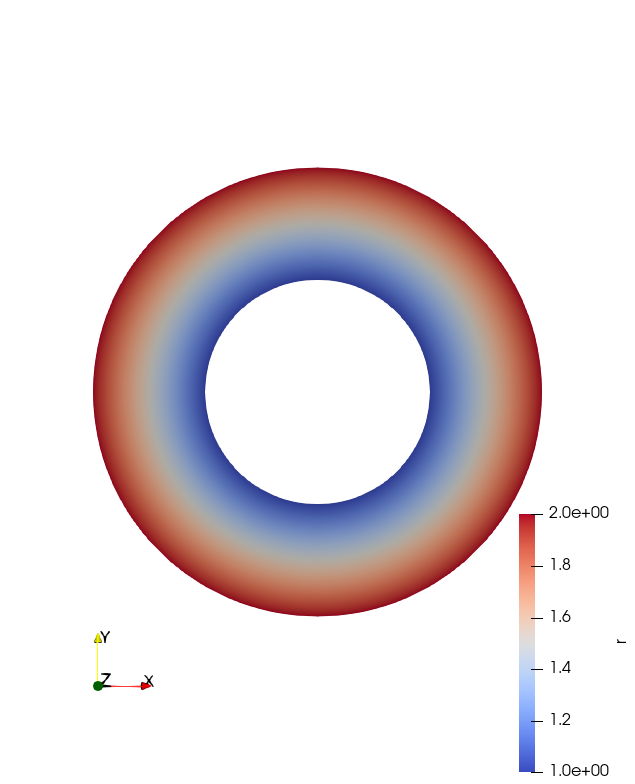
\includegraphics[width=5.6cm]{./python_codes/fieldstone_151/images/r}
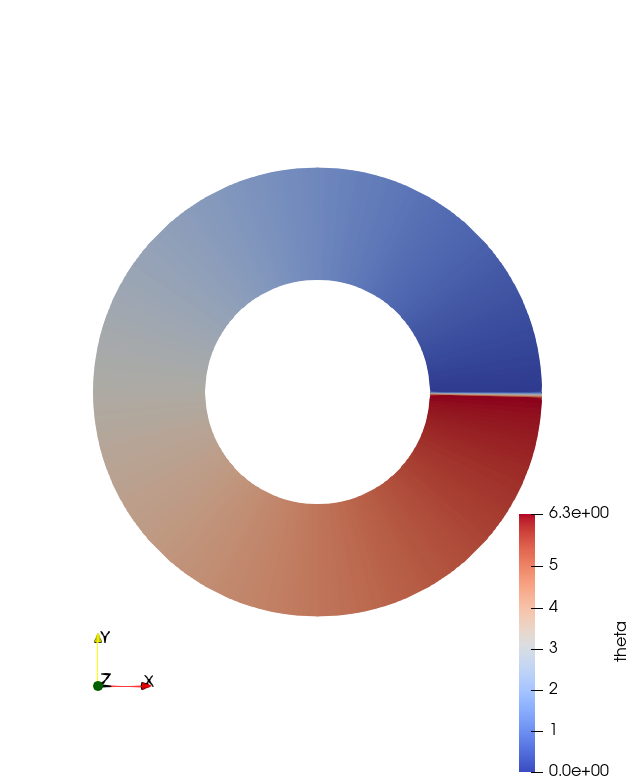
\includegraphics[width=5.6cm]{./python_codes/fieldstone_151/images/theta}\\
{\captionfont Mesh, $r$ and $\theta$ coordinates.}
\end{center}

\begin{center}
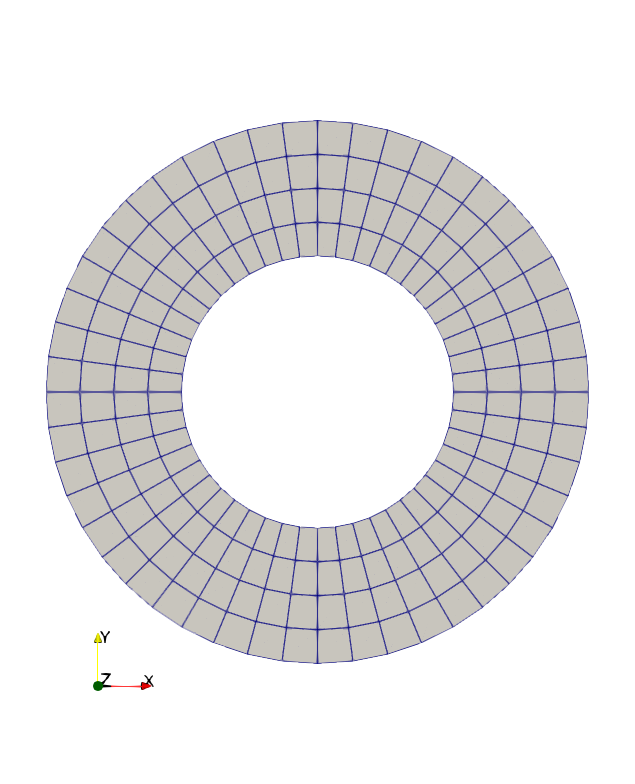
\includegraphics[width=6cm]{./python_codes/fieldstone_151/images/mesh1}
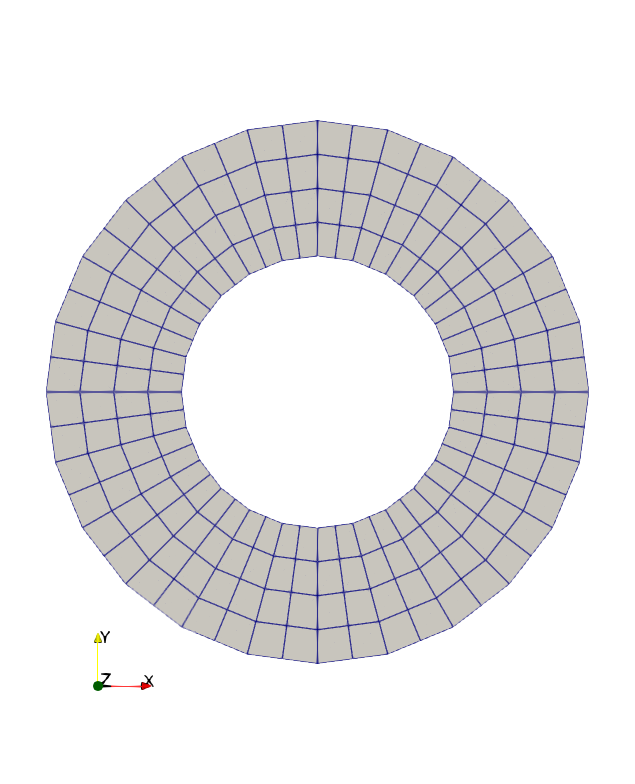
\includegraphics[width=6cm]{./python_codes/fieldstone_151/images/mesh2}\\
{\captionfont Left: {\python trapezes=0}; right:   {\python trapezes=1}.}
\end{center}

\noindent The goal of this \stone is twofold:
\begin{itemize}
\item test the implementation of the free slip boundary conditions algorithms,
\item explore the differences between straight edge elelements vs curved ones.
\end{itemize}






\newpage
%%%%%%%%%%%%%%%%%%%%%%%%%%%%%%%%%%%%%%%%%%%%%%%%%%%%%%%%%%%%%
\section*{Method 1: rotating elemental matrices}

This is explained in Section~\ref{MMM-ss:fsbc_annulus}.

%%%%%%%%%%%%%%%%%%%%%%%%%%%%%%%%%%%%%%%%%%%%%%%%%%%%%%%%%%%%%
\section*{Method 2: constraints applied to elemental matrix}

After asking W. Bangerth about the deal.II strategy for such boundary conditions 
his email answer was

\begin{verbatim}
----------------------------------------------------------
It's this function:

https://dealii.org/developer/doxygen/deal.II/group__constraints.html#gae3b53d69bd7afe08f0d033497833938e

In short, we compute constraints on individual nodes that correspond to the
  u.n = 0
constraint. In 2d, you get something like
  ux*nx + uy*ny = 0
which you convert into a constraint of the kind
  ux = - uy*ny/nx
or
  uy = - ux*nx/ny
depending on whether nx>ny or nx<ny, for numerical stability.
----------------------------------------------------------
\end{verbatim}

What follows is mine only.



\[
\left(
\begin{array}{cc}
\K_e & \G_e \\
\G_e^T & 0
\end{array}
\right)
\cdot
\left(
\begin{array}{c}
\vec{V} \\
\vec{P}
\end{array}
\right)
=\left(
\begin{array}{c}
\vec{f} \\ \vec{h}
\end{array}
\right)
\]
Let us assume that node 2 is on the boundary and we therefore wish to 
impose $\vec{v}_2\cdot \vec{n}=0$, or $u_2 n_x + v_2 n_y =0$.

The equation above writes (for simplicity we take $m_v=4$ and $m_p=3$ which does not correspond to a real FE pair) 
with $K_e$ of size $8\times 8$ and $G_e$ of size $8\times 3$ in 2D:
{\small
\[
\begin{array}{ccccccccccccc}
K_{11} u_1 &+ K_{12} v_1 &+ K_{13} u_2 &+ K_{14} v_2 &+ K_{15} u_3 &+ K_{16} v_3 &+ K_{17}u_4  &+ K_{18}v_4  
&+ G_{11}p_1 &+ G_{12} p_2 &+ G_{13} p_3 & =  f_1 \\
K_{21} u_1 &+ K_{22} v_1 &+ K_{23} u_2 &+ K_{24} v_2 &+ K_{25} u_3 &+ K_{26} v_3 &+ K_{27}u_4  &+ K_{28}v_4  
&+ G_{21}p_1 &+ G_{22} p_2 &+ G_{23} p_3 & =  f_2 \\
K_{31} u_1 &+ K_{32} v_1 &+ K_{33} u_2 &+ K_{34} v_2 &+ K_{35} u_3 &+ K_{36} v_3 &+ K_{37}u_4  &+ K_{38}v_4  
&+ G_{31}p_1 &+ G_{32} p_2 &+ G_{33} p_3 & =  f_3 \\
K_{41} u_1 &+ K_{42} v_1 &+ K_{43} u_2 &+ K_{44} v_2 &+ K_{45} u_3 &+ K_{46} v_3 &+ K_{47}u_4  &+ K_{48}v_4  
&+ G_{41}p_1 &+ G_{42} p_2 &+ G_{43} p_3 & =  f_4 \\
K_{51} u_1 &+ K_{52} v_1 &+ K_{53} u_2 &+ K_{54} v_2 &+ K_{55} u_3 &+ K_{56} v_3 &+ K_{57}u_4  &+ K_{58}v_4  
&+ G_{51}p_1 &+ G_{52} p_2 &+ G_{53} p_3 & =  f_5 \\
K_{61} u_1 &+ K_{62} v_1 &+ K_{63} u_2 &+ K_{64} v_2 &+ K_{65} u_3 &+ K_{66} v_3 &+ K_{67}u_4  &+ K_{68}v_4  
&+ G_{61}p_1 &+ G_{62} p_2 &+ G_{63} p_3 & =  f_6 \\
K_{71} u_1 &+ K_{72} v_1 &+ K_{73} u_2 &+ K_{74} v_2 &+ K_{75} u_3 &+ K_{76} v_3 &+ K_{77}u_4  &+ K_{78}v_4  
&+ G_{71}p_1 &+ G_{72} p_2 &+ G_{73} p_3 & =  f_7 \\
K_{81} u_1 &+ K_{82} v_1 &+ K_{83} u_2 &+ K_{84} v_2 &+ K_{85} u_3 &+ K_{86} v_3 &+ K_{87}u_4  &+ K_{88}v_4  
&+ G_{81}p_1 &+ G_{82} p_2 &+ G_{83} p_3 & =  f_8 \\
G_{11}u_1 &+ G_{21}v_1 &+ G_{31}u_2 &+ G_{41}v_2 &+ G_{51}u_3 &+ G_{61}v_3 &+ G_{71}u_4 &+ G_{81}v_4 &+0&+0&+0&= h_1 \\
G_{12}u_1 &+ G_{22}v_1 &+ G_{32}u_2 &+ G_{42}v_2 &+ G_{52}u_3 &+ G_{62}v_3 &+ G_{72}u_4 &+ G_{82}v_4 &+0&+0&+0&= h_2 \\
G_{13}u_1 &+ G_{23}v_1 &+ G_{33}u_2 &+ G_{43}v_2 &+ G_{53}u_3 &+ G_{63}v_3 &+ G_{73}u_4 &+ G_{83}v_4 &+0&+0&+0&= h_3
\end{array}
\]
}
We must now find a way to include the contraint above in these equations.
Typically we usually have $v_2=v_{bc}$ and the system above is transformed as follows
{\small
\[
\begin{array}{lllllllllllll}
K_{11} u_1 &+ K_{12} v_1 &+ K_{13} u_2 &+ 0 &+ K_{15} u_3 &+ K_{16} v_3 &+ K_{17}u_4  &+ K_{18}v_4  
&+ G_{11}p_1 &+ G_{12} p_2 &+ G_{13} p_3 & =  f_1 -K_{14} v_{bc}\\
K_{21} u_1 &+ K_{22} v_1 &+ K_{23} u_2 &+ 0 &+ K_{25} u_3 &+ K_{26} v_3 &+ K_{27}u_4  &+ K_{28}v_4  
&+ G_{21}p_1 &+ G_{22} p_2 &+ G_{23} p_3 & =  f_2 -K_{24} v_{bc}\\
K_{31} u_1 &+ K_{32} v_1 &+ K_{33} u_2 &+ 0 &+ K_{35} u_3 &+ K_{36} v_3 &+ K_{37}u_4  &+ K_{38}v_4  
&+ G_{21}p_1 &+ G_{32} p_2 &+ G_{33} p_3 & =  f_3 -K_{34} v_{bc}\\
0  &+ 0  &+ 0  &+ K_{44} v_2 &+ 0 &+ 0 &+ 0  &+ 0  
&+ 0 &+ 0 &+ 0 & = & K_{44}v_{bc} \\
K_{51} u_1 &+ K_{52} v_1 &+ K_{53} u_2 &+ 0 &+ K_{55} u_3 &+ K_{56} v_3 &+ K_{57}u_4  &+ K_{58}v_4  
&+ G_{21}p_1 &+ G_{52} p_2 &+ G_{53} p_3 & =  f_5 -K_{54} v_{bc}\\
K_{61} u_1 &+ K_{62} v_1 &+ K_{63} u_2 &+ 0 &+ K_{65} u_3 &+ K_{66} v_3 &+ K_{67}u_4  &+ K_{68}v_4  
&+ G_{21}p_1 &+ G_{62} p_2 &+ G_{63} p_3 & =  f_6 -K_{64} v_{bc}\\
K_{71} u_1 &+ K_{72} v_1 &+ K_{73} u_2 &+ 0 &+ K_{75} u_3 &+ K_{76} v_3 &+ K_{77}u_4  &+ K_{78}v_4  
&+ G_{21}p_1 &+ G_{72} p_2 &+ G_{73} p_3 & =  f_7 -K_{74} v_{bc}\\
K_{81} u_1 &+ K_{82} v_1 &+ K_{83} u_2 &+ 0 &+ K_{85} u_3 &+ K_{86} v_3 &+ K_{87}u_4  &+ K_{88}v_4  
&+ G_{21}p_1 &+ G_{82} p_2 &+ G_{83} p_3 & =  f_8 -K_{84} v_{bc}\\
G_{11}u_1 &+ G_{21}v_1 &+ G_{31}u_2 &+ 0 &+ G_{51}u_3 &+ G_{61}v_3 &+ G_{71}u_4 &+ G_{81}v_4 &+0&+0&+0&= h_1 -G_{41}v_{bc}\\
G_{12}u_1 &+ G_{22}v_1 &+ G_{32}u_2 &+ 0 &+ G_{52}u_3 &+ G_{62}v_3 &+ G_{72}u_4 &+ G_{82}v_4 &+0&+0&+0&= h_2 -G_{42}v_{bc}\\
G_{13}u_1 &+ G_{23}v_1 &+ G_{33}u_2 &+ 0 &+ G_{53}u_3 &+ G_{63}v_3 &+ G_{73}u_4 &+ G_{83}v_4 &+0&+0&+0&= h_3 -G_{43}v_{bc}
\end{array}
\]
}
This approach yields an elemental Stokes matrix that is still strictly symmetric. Since we only build $G_{e}$ (and not $G_e^T$) 
in the code then zeroing a line in $G_e$ means zeroing a line in $G_e^T$ so the approach above reconciles this pb.

If $v_{bc}=0$ then we obtain
{\small
\[
\begin{array}{lllllllllllll}
K_{11} u_1 &+ K_{12} v_1 &+ K_{13} u_2 &+ 0 &+ K_{15} u_3 &+ K_{16} v_3 &+ K_{17}u_4  &+ K_{18}v_4  
&+ G_{11}p_1 &+ G_{12} p_2 &+ G_{13} p_3 & =  f_1 \\
K_{21} u_1 &+ K_{22} v_1 &+ K_{23} u_2 &+ 0 &+ K_{25} u_3 &+ K_{26} v_3 &+ K_{27}u_4  &+ K_{28}v_4  
&+ G_{21}p_1 &+ G_{22} p_2 &+ G_{23} p_3 & =  f_2 \\
K_{31} u_1 &+ K_{32} v_1 &+ K_{33} u_2 &+ 0 &+ K_{35} u_3 &+ K_{36} v_3 &+ K_{37}u_4  &+ K_{38}v_4  
&+ G_{21}p_1 &+ G_{32} p_2 &+ G_{33} p_3 & =  f_3 \\
0  &+ 0  &+ 0  &+ K_{44} v_2 &+ 0 &+ 0 &+ 0  &+ 0  
&+ 0 &+ 0 &+ 0 & =  0 \\
K_{51} u_1 &+ K_{52} v_1 &+ K_{53} u_2 &+ 0 &+ K_{55} u_3 &+ K_{56} v_3 &+ K_{57}u_4  &+ K_{58}v_4  
&+ G_{21}p_1 &+ G_{52} p_2 &+ G_{53} p_3 & =  f_5 \\
K_{61} u_1 &+ K_{62} v_1 &+ K_{63} u_2 &+ 0 &+ K_{65} u_3 &+ K_{66} v_3 &+ K_{67}u_4  &+ K_{68}v_4  
&+ G_{21}p_1 &+ G_{62} p_2 &+ G_{63} p_3 & =  f_6 \\
K_{71} u_1 &+ K_{72} v_1 &+ K_{73} u_2 &+ 0 &+ K_{75} u_3 &+ K_{76} v_3 &+ K_{77}u_4  &+ K_{78}v_4  
&+ G_{21}p_1 &+ G_{72} p_2 &+ G_{73} p_3 & =  f_7 \\
K_{81} u_1 &+ K_{82} v_1 &+ K_{83} u_2 &+ 0 &+ K_{85} u_3 &+ K_{86} v_3 &+ K_{87}u_4  &+ K_{88}v_4  
&+ G_{21}p_1 &+ G_{82} p_2 &+ G_{83} p_3 & =  f_8 \\
G_{11}u_1 &+ G_{21}v_1 &+ G_{31}u_2 &+ 0 &+ G_{51}u_3 &+ G_{61}v_3 &+ G_{71}u_4 &+ G_{81}v_4 &+0&+0&+0&= h_1 \\
G_{12}u_1 &+ G_{22}v_1 &+ G_{32}u_2 &+ 0 &+ G_{52}u_3 &+ G_{62}v_3 &+ G_{72}u_4 &+ G_{82}v_4 &+0&+0&+0&= h_2 \\
G_{13}u_1 &+ G_{23}v_1 &+ G_{33}u_2 &+ 0 &+ G_{53}u_3 &+ G_{63}v_3 &+ G_{73}u_4 &+ G_{83}v_4 &+0&+0&+0&= h_3 
\end{array}
\]
}

Let us now turn to free slip and start with $v_2=-u_2 n_x/n_y$. Then we could write:
{\small
\[
\begin{array}{lllllllllllll}
K_{11} u_1 &+ K_{12} v_1 &+ (K_{13}-\frac{n_x}{n_y}K_{14}) u_2 &+ 0 &+ K_{15} u_3 &+ K_{16} v_3 &+ K_{17}u_4  &+ K_{18}v_4  
&+ G_{11}p_1 &+ G_{12} p_2 &+ G_{13} p_3 & =  f_1 \\
K_{21} u_1 &+ K_{22} v_1 &+ (K_{23}-\frac{n_x}{n_y}K_{24}) u_2 &+ 0 &+ K_{25} u_3 &+ K_{26} v_3 &+ K_{27}u_4  &+ K_{28}v_4  
&+ G_{21}p_1 &+ G_{22} p_2 &+ G_{23} p_3 & =  f_2 \\
K_{31} u_1 &+ K_{32} v_1 &+ (K_{33}-\frac{n_x}{n_y}K_{34}) u_2 &+ 0 &+ K_{35} u_3 &+ K_{36} v_3 &+ K_{37}u_4  &+ K_{38}v_4  
&+ G_{31}p_1 &+ G_{32} p_2 &+ G_{33} p_3 & =  f_3 \\
0 &+ 0 & +K_{44}\frac{n_x}{n_y} u_2 &+ K_{44} v_2 &+ 0 &+ 0 &+ 0  &+ 0  
&+ 0 &+ 0 &+ 0 & =  0 \\
K_{51} u_1 &+ K_{52} v_1 &+ (K_{53}-\frac{n_x}{n_y}K_{54}) u_2 &+ 0 &+ K_{55} u_3 &+ K_{56} v_3 &+ K_{57}u_4  &+ K_{58}v_4  
&+ G_{51}p_1 &+ G_{52} p_2 &+ G_{53} p_3 & =  f_5 \\
K_{61} u_1 &+ K_{62} v_1 &+ (K_{63}-\frac{n_x}{n_y}K_{64}) u_2 &+ 0 &+ K_{65} u_3 &+ K_{66} v_3 &+ K_{67}u_4  &+ K_{68}v_4  
&+ G_{61}p_1 &+ G_{62} p_2 &+ G_{63} p_3 & =  f_6 \\
K_{71} u_1 &+ K_{72} v_1 &+ (K_{73}-\frac{n_x}{n_y}K_{74}) u_2 &+ 0 &+ K_{75} u_3 &+ K_{76} v_3 &+ K_{77}u_4  &+ K_{78}v_4  
&+ G_{71}p_1 &+ G_{72} p_2 &+ G_{73} p_3 & =  f_7 \\
K_{81} u_1 &+ K_{82} v_1 &+ (K_{83}-\frac{n_x}{n_y}K_{84}) u_2 &+ 0 &+ K_{85} u_3 &+ K_{86} v_3 &+ K_{87}u_4  &+ K_{88}v_4  
&+ G_{81}p_1 &+ G_{82} p_2 &+ G_{83} p_3 & =  f_8 \\
G_{11}u_1 &+ G_{21}v_1 &+ (G_{31}-\frac{n_x}{n_y}G_{41})u_2 &+0  &+ G_{51}u_3 &+ G_{61}v_3 &+ G_{71}u_4 &+ G_{81}v_4 &+0&+0&+0&= h_1 \\
G_{12}u_1 &+ G_{22}v_1 &+ (G_{32}-\frac{n_x}{n_y}G_{42})u_2 &+0  &+ G_{52}u_3 &+ G_{62}v_3 &+ G_{72}u_4 &+ G_{82}v_4 &+0&+0&+0&= h_2 \\
G_{13}u_1 &+ G_{23}v_1 &+ (G_{33}-\frac{n_x}{n_y}G_{43})u_2 &+0  &+ G_{53}u_3 &+ G_{63}v_3 &+ G_{73}u_4 &+ G_{83}v_4 &+0&+0&+0&= h_3
\end{array}
\]
}
which is not very useful since the symmetry has been destroyed. Note that when $n_x\rightarrow 0$ 
then we recover the system above.

May be the simplest approach is then to do
{\small
\[
\begin{array}{lllllllllllll}
K_{11} u_1 &+ K_{12} v_1 &+ K_{13} u_2 &+ K_{14} v_2 &+ K_{15} u_3 &+ K_{16} v_3 &+ K_{17}u_4  &+ K_{18}v_4  
&+ G_{11}p_1 &+ G_{12} p_2 &+ G_{13} p_3 & =  f_1 \\
K_{21} u_1 &+ K_{22} v_1 &+ K_{23} u_2 &+ K_{24} v_2 &+ K_{25} u_3 &+ K_{26} v_3 &+ K_{27}u_4  &+ K_{28}v_4  
&+ G_{21}p_1 &+ G_{22} p_2 &+ G_{23} p_3 & =  f_2 \\
K_{31} u_1 &+ K_{32} v_1 &+ K_{33} u_2 &+ K_{34} v_2 &+ K_{35} u_3 &+ K_{36} v_3 &+ K_{37}u_4  &+ K_{38}v_4  
&+ G_{31}p_1 &+ G_{32} p_2 &+ G_{33} p_3 & =  f_3 \\
0 &+ 0 & +K_{44}\frac{n_x}{n_y} u_2 &+ K_{44} v_2 &+ 0 &+ 0 &+ 0  &+ 0  
&+ 0 &+ 0 &+ 0 & =  0 \\
K_{51} u_1 &+ K_{52} v_1 &+ K_{53} u_2 &+ K_{54} v_2 &+ K_{55} u_3 &+ K_{56} v_3 &+ K_{57}u_4  &+ K_{58}v_4  
&+ G_{51}p_1 &+ G_{52} p_2 &+ G_{53} p_3 & =  f_5 \\
K_{61} u_1 &+ K_{62} v_1 &+ K_{63} u_2 &+ K_{64} v_2 &+ K_{65} u_3 &+ K_{66} v_3 &+ K_{67}u_4  &+ K_{68}v_4  
&+ G_{61}p_1 &+ G_{62} p_2 &+ G_{63} p_3 & =  f_6 \\
K_{71} u_1 &+ K_{72} v_1 &+ K_{73} u_2 &+ K_{74} v_2 &+ K_{75} u_3 &+ K_{76} v_3 &+ K_{77}u_4  &+ K_{78}v_4  
&+ G_{71}p_1 &+ G_{72} p_2 &+ G_{73} p_3 & =  f_7 \\
K_{81} u_1 &+ K_{82} v_1 &+ K_{83} u_2 &+ K_{84} v_2 &+ K_{85} u_3 &+ K_{86} v_3 &+ K_{87}u_4  &+ K_{88}v_4  
&+ G_{81}p_1 &+ G_{82} p_2 &+ G_{83} p_3 & =  f_8 \\
G_{11}u_1 &+ G_{21}v_1 &+ G_{31}u_2 &+ G_{41}v_2 &+ G_{51}u_3 &+ G_{61}v_3 &+ G_{71}u_4 &+ G_{81}v_4 &+0&+0&+0&= h_1 \\
G_{12}u_1 &+ G_{22}v_1 &+ G_{32}u_2 &+ G_{42}v_2 &+ G_{52}u_3 &+ G_{62}v_3 &+ G_{72}u_4 &+ G_{82}v_4 &+0&+0&+0&= h_2 \\
G_{13}u_1 &+ G_{23}v_1 &+ G_{33}u_2 &+ G_{43}v_2 &+ G_{53}u_3 &+ G_{63}v_3 &+ G_{73}u_4 &+ G_{83}v_4 &+0&+0&+0&= h_3
\end{array}
\]
}
but it means that after imposing the b.c. I end up with a system like

\[
\left(
\begin{array}{cc}
K_e & G_1 \\
G_1^T & 0
\end{array}
\right)
\cdot
\left(
\begin{array}{c}
\vec{V} \\
\vec{P}
\end{array}
\right)
=\left(
\begin{array}{c}
\vec{f} \\ \vec{h}
\end{array}
\right)
\]

After writing \& sending my doubts to Wolfgang:
\begin{verbatim}
C: My instinct(memory?) tells me that having the discretised gradient and
divergence operators not being the transpose of one another (after applying
boundary conditions) is wrong. Is my hunch correct? If so, what is the common
procedure? 
W: Yes, you need to keep things symmetric.
If you have constraints that couple multiple DoFs, the procedure is
substantially more complex. I've never really seen a good description of how
this is done (even though it's been done for decades), so I wrote it up a few
years ago. Take a look at section 5 here:
https://www.math.colostate.edu/~bangerth/publications/2006-hp.pdf
\end{verbatim}
This publication is: \fullcite{baka09}.

This therefore means that this approach is not viable and {\python fs\_method=2} 
should not be used. 

%%%%%%%%%%%%%%%%%%%%%%%%%%%%%%%%%%%%%%%%%%%%%%%%%%%%%%%%%%%%%
\section*{method 3: constraints via Lagrange multipliers}

Once assembled (without the free slip constraints) the Stokes system 
is 
\[
\left(
\begin{array}{cc}
\K & \G \\
\G^T & 0
\end{array}
\right)
\cdot
\left(
\begin{array}{c}
\vec{V} \\
\vec{P}
\end{array}
\right)
=\left(
\begin{array}{c}
\vec{f} \\ \vec{h}
\end{array}
\right)
\]
Since we wish to impose free slip at all nodes on the outer surface\footnote{We restrict ourselves to the outer boundary} 
of the annulus by means of Lagrange mutlipliers the new system will 
look like
\[
\left(
\begin{array}{ccc}
\K & \G & \mathbb{L}\\
\G^T & 0 &0 \\
\mathbb{L}^T & 0 & 0
\end{array}
\right)
\cdot
\left(
\begin{array}{c}
\vec{V} \\
\vec{P} \\
\vec{\Lambda}
\end{array}
\right)
=\left(
\begin{array}{c}
\vec{f} \\ \vec{h} \\ \vec{0}
\end{array}
\right)
\]
The vector $\vec\Lambda$ is $N_{lm}$ long where 
$N_{lm}$ is the number of nodes on the outer surface.
Since the constraints do not involve the pressure dofs 
there is only one block added to the global matrix, 
coined $\mathbb{L}$ of size $(ndofV*N_V) \times N_{lm}$.

The total size of the Stokes matrix is then $NfemV+NfemP+N_{lm}$.
The non zero entries of $\mathbb{L}$ are obtained by 
looping over all surface nodes, computing the normal vector $(n_x,n_y)$ there, and 
writing $n_x$ and $n_y$ in $\mathbb{L}$ at the right line (corresponding to the 
surface node identity) so that $n_x u + n_y v = 0$:
\begin{lstlisting}
counter=NfemV+NfemP
for i in range(0,nnp):
    if surface[i]:
       A_sparse[counter,2*i  ]=nx[i]
       A_sparse[counter,2*i+1]=ny[i]
       A_sparse[2*i  ,counter]=nx[i]
       A_sparse[2*i+1,counter]=ny[i]
       counter+=1
\end{lstlisting}

This turns out to be a very simple method to implement. However, it has the disadvantage that 
the Stokes matrix is now larger and contains yet another zero block on the diagonal.

Q: what is the meaning of the vector $\Lambda$ that we recover after solving the system?

\newpage
%%%%%%%%%%%%%%%%%%%%%%%%%%%%%%%%%%%%%%%%%%%%%%%%%%%%%%%%%%%%%%%%%%%%%%%%%%%%%%%%%%%%%%%%%%%%%%%%%%%
\section*{Computing the normal vector}

In the case of an annulus, the normal to the surface is easily calculated. If a node $i$
has an associated angle $\theta_i$, then its normal vector is $\vec{n}_i=(\cos\theta_i,\sin\theta_i)$.
This simply translates as follows in the code:

\begin{lstlisting}
nx1=np.zeros(NV,dtype=np.float64) 
ny1=np.zeros(NV,dtype=np.float64) 
for i in range(0,NV):
    if rV[i]/R2>1-eps:
       nx1[i]=np.cos(theta[i])
       ny1[i]=np.sin(theta[i])
\end{lstlisting}

However, as explained in \textcite{ensg82}, the normal vector at a node $i$ can be computed using the 
basis function derivatives:
\begin{eqnarray}
n_{x,i} &=& \frac{1}{n_i}\int_\Omega \frac{\partial \bN_i}{\partial x} dV \nn\\
n_{y,i} &=& \frac{1}{n_i}\int_\Omega \frac{\partial \bN_i}{\partial y} dV \nn
\end{eqnarray}
with 
\[
n_i = \left[
\left(\int_\Omega \frac{\partial \bN_i}{\partial x} dV\right)^2 +
\left(\int_\Omega \frac{\partial \bN_i}{\partial y} dV\right)^2 
\right]^{1/2}
\]
This second method yields the nodal fields
\begin{lstlisting}
nx2=np.zeros(NV,dtype=np.float64) 
ny2=np.zeros(NV,dtype=np.float64) 
\end{lstlisting}
and the {\python normal\_type} indicates which of the two normal vectors is to be 
used.  

Actually, when computing $\vec{n}_1$ and $\vec{n}_2$ on the outer surface of the annulus we find 
not so surprisingly that the two vectors are nearly identical (the difference is basically machine precision):

\begin{center}
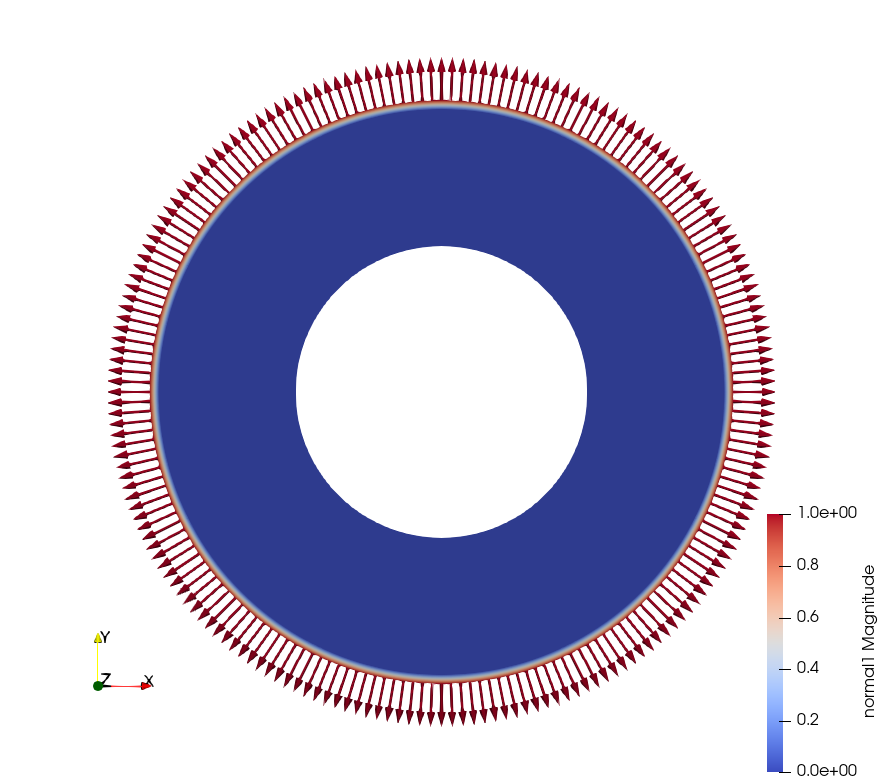
\includegraphics[width=5.7cm]{python_codes/fieldstone_151/images/n1}
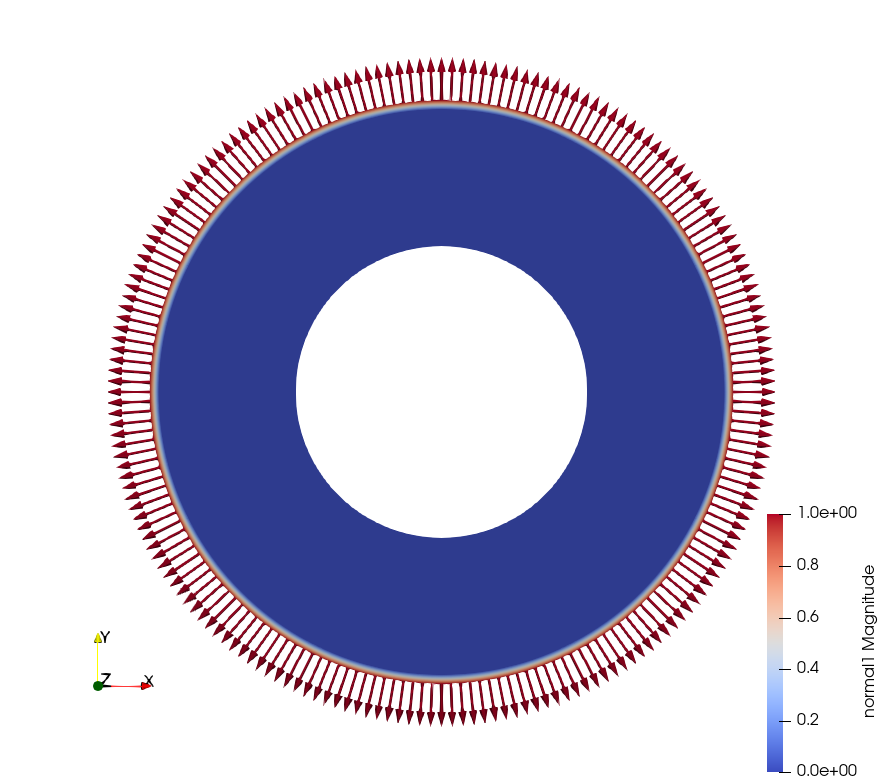
\includegraphics[width=5.7cm]{python_codes/fieldstone_151/images/n2}
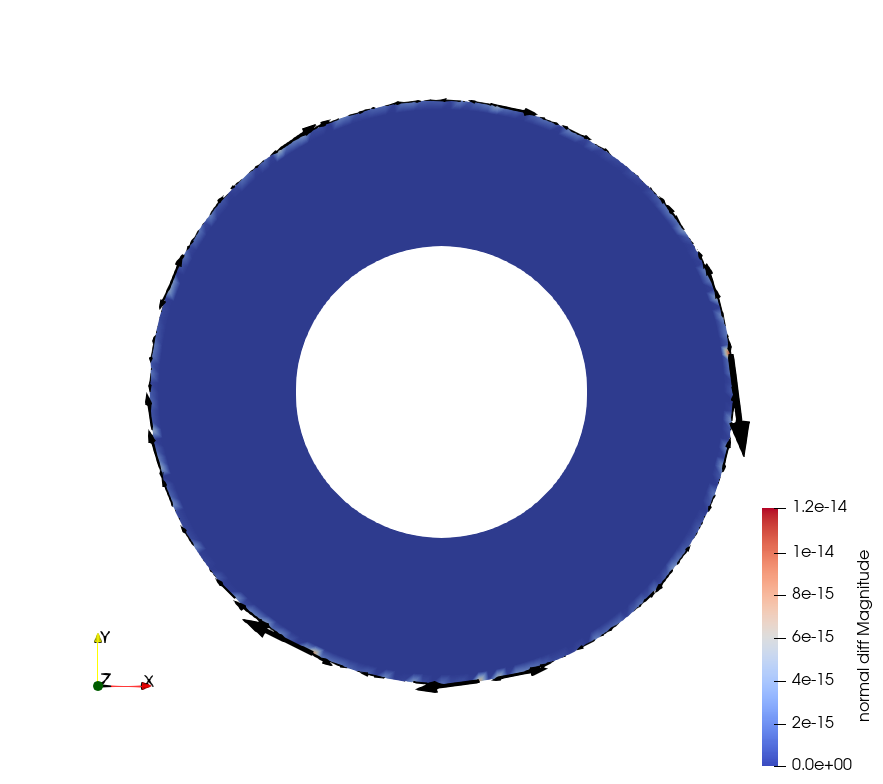
\includegraphics[width=5.7cm]{python_codes/fieldstone_151/images/n12}\\
{\captionfont Mesh $8\times 96$ elements.}
\end{center}

In what follows models are run with $\vec{n}_1$.


\newpage
%%%%%%%%%%%%%%%%%%%%%%%%%%%%%%%%%%%%%%%%%%%%%%%%%%%%%%%%%%%%%%%%%%%%%%%%%%%%%%%%%%%%%%%%%%%%%%%%%%%
\section*{Various benchmarks/tests}

In what follows we set $R_1=1$ and $R_2=2$. Unless otherwise specified we also set $\rho=1$
and $\eta=1$. The following tests are such that there is no rotational nullspace.
Note that the argument $n$ passed as argument to the code is the number of $Q_1$ 
elements in the radial direction.

%%%%%%%%%%%%%%%%%%%%%%%%%%%%%%%%%%%%%%%%%%%
\subsection*{test \#1: the aquarium - no slip}

Results are obtained by running {\tt script1}. Boundary conditions are 
no slip on the surface and the cmb. 
The analytical solution is a zero velocity field and an hydrostatic pressure field.
The following figures show the error convergence for both velocity and pressure.

\begin{center}
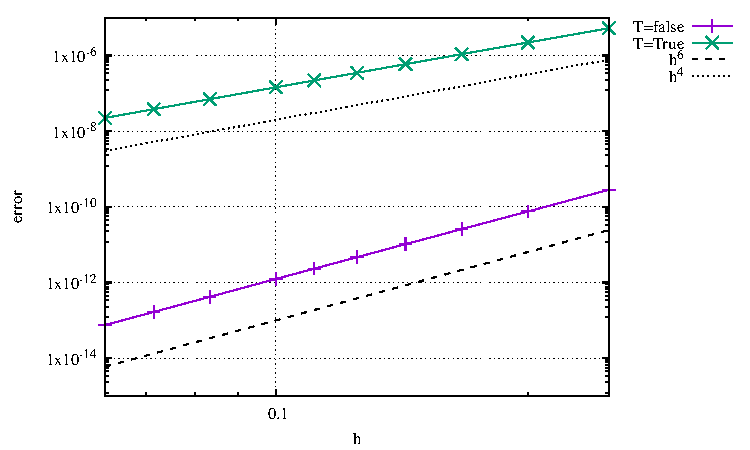
\includegraphics[width=6cm]{python_codes/fieldstone_151/results/test1/errv}
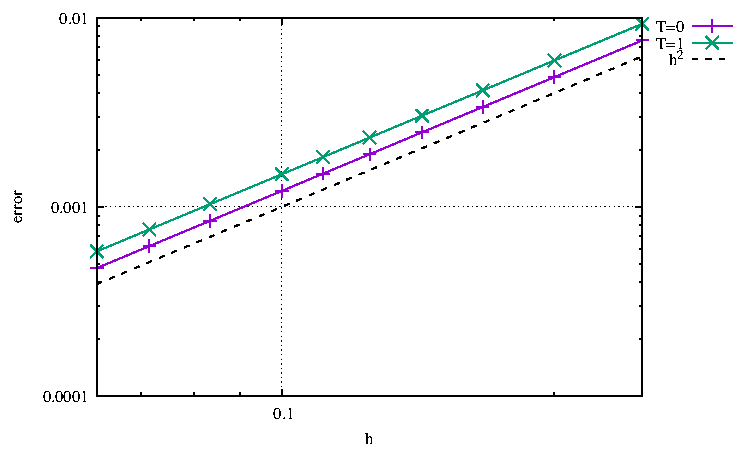
\includegraphics[width=6cm]{python_codes/fieldstone_151/results/test1/errp}\\
{\captionfont T=1 means {\python trapezes=True}.}
\end{center}

We obtain a supra-convergence for velocity and quadratic convergence for pressure.
This experiment serves as a reference for the next one.

%%%%%%%%%%%%%%%%%%%%%%%%%%%%%%%%%%%%%%%%%%%
\subsection*{test \#2: the aquarium - free slip}

Results are obtained by running {\tt script2}. 
This is the same experiment as test 1, but we now prescribe free slip on the 
outer surface by means of method 1 or 3. The analytical solution is identical 
and we recover near identical results as before, for both methods.

\begin{center}
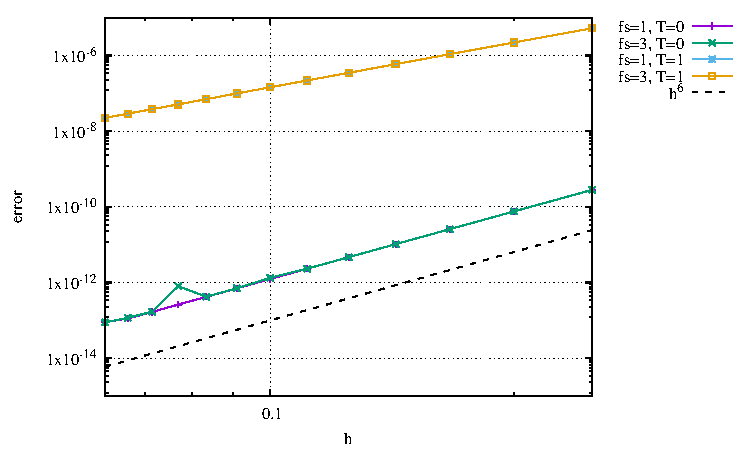
\includegraphics[width=6cm]{python_codes/fieldstone_151/results/test2/errv}
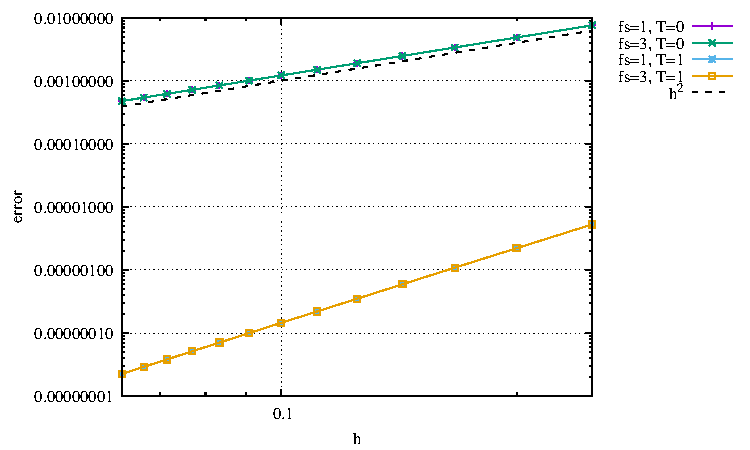
\includegraphics[width=6cm]{python_codes/fieldstone_151/results/test2/errp}\\
{\captionfont T=1 means {\python trapezes=True}.}
\end{center}

Unsurprisingly we also find that not using trapezoidal elements yields a 
much higher accuracy for the volume of the domain:
\begin{center}
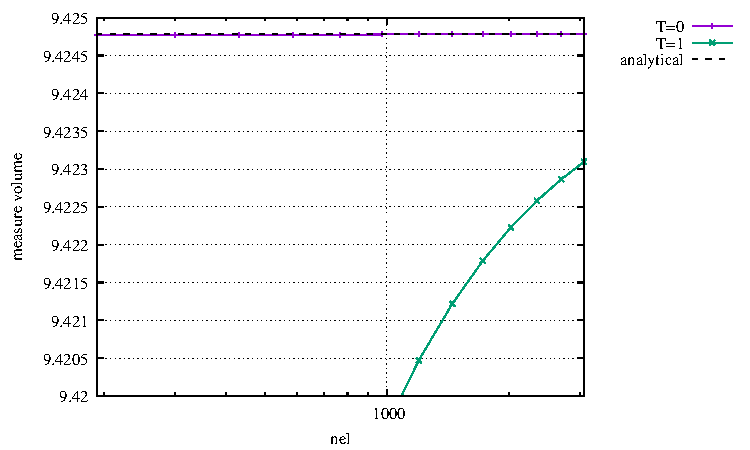
\includegraphics[width=6cm]{python_codes/fieldstone_151/results/test2/areas}\\
{\captionfont total area of the domain measured by means of Gauss integration.
T=1 means {\python trapezes=True}.}
\end{center}



%%%%%%%%%%%%%%%%%%%%%%%%%%%%%%%%%%%%%%%
\subsection*{test \#3: shearing - no slip}

Results are obtained by running {\tt script3}. Boundary conditions are 
no slip on the surface and a prescribed constant velocity $\upnu_{bc}=1$ tangent 
to the inner boundary.
The analytical solution is hydrostatic pressure and a rotational velocity going from 
$1$ at the cmb to 0 on the outer surface

TODO




%%%%%%%%%%%%%%%%%%%%%%%%%%%%%%%%%%%%%%%%%
\subsection*{test \#4: shearing - free slip}

Results are obtained by running {\tt script4}. Boundary conditions are 
free slip on the surface and a prescribed constant velocity $\upnu_{bc}=1$ tangent 
to the inner boundary.

The analytical solution is described in Section~\ref{MMM-ss:ankbc}.
It is a hydrostatic pressure and a rotational velocity given by $\vec{\upnu}=\upnu_r \vec{e}_r + \upnu_\theta \vec{e}_\theta = r \; \vec{e}_\theta$.
Turning to Section~\ref{MMM-ss:srpc}:

\begin{eqnarray}
\dot\varepsilon_{rr}  &=& \frac{\partial \upnu_r}{\partial r}  = 0\\
\dot\varepsilon_{\theta\theta}  &=& \frac{\upnu_r}{r} + \frac{1}{r} \frac{\partial \upnu_\theta}{\partial \theta} =0 \\
\dot\varepsilon_{\theta r} = \dot\varepsilon_{r\theta}  &=& \frac{1}{2} \left(   \frac{\partial \upnu_\theta}{\partial r} - \frac{\upnu_\theta}{r} 
+\frac{1}{r} \frac{\partial \upnu_r}{\partial \theta}  \right)  = \frac12 (1-1) =0
\end{eqnarray}


\begin{center}
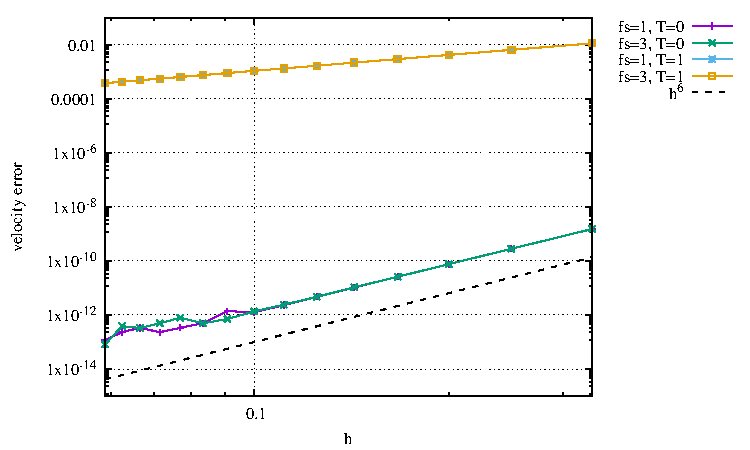
\includegraphics[width=5.6cm]{python_codes/fieldstone_151/results/test4/errv}
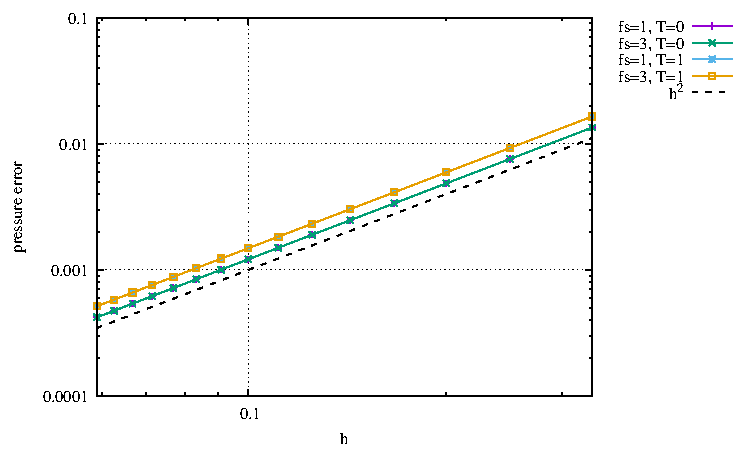
\includegraphics[width=5.6cm]{python_codes/fieldstone_151/results/test4/errp}
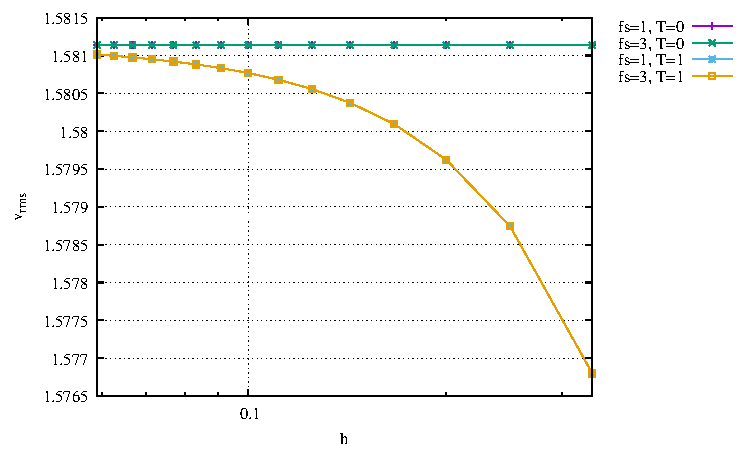
\includegraphics[width=5.6cm]{python_codes/fieldstone_151/results/test4/vrms}\\
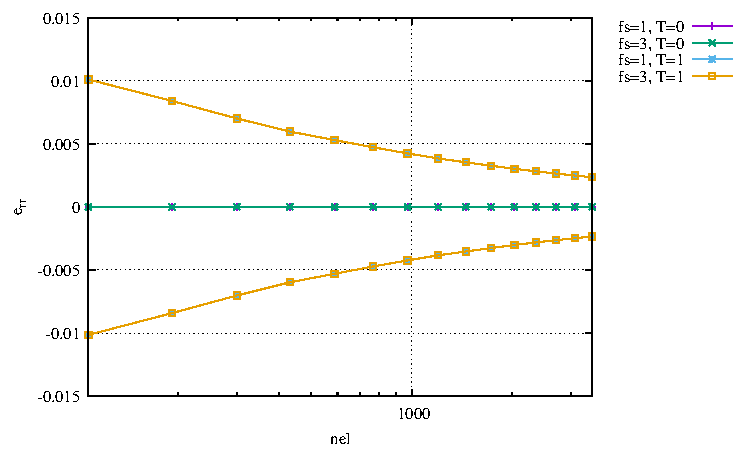
\includegraphics[width=5.6cm]{python_codes/fieldstone_151/results/test4/e_rr}
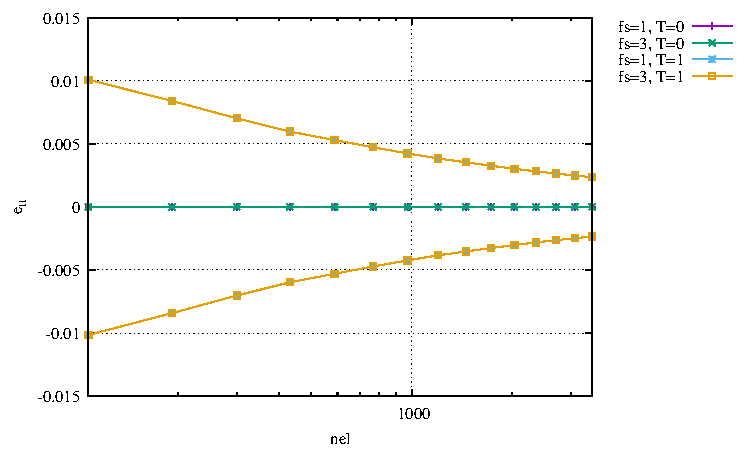
\includegraphics[width=5.6cm]{python_codes/fieldstone_151/results/test4/e_tt}
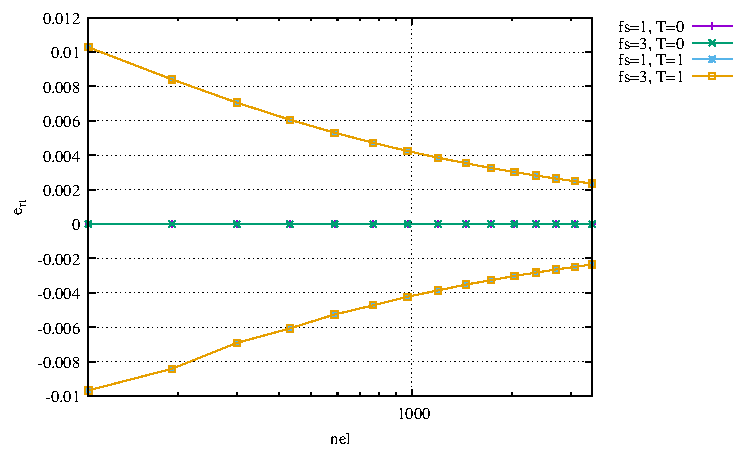
\includegraphics[width=5.6cm]{python_codes/fieldstone_151/results/test4/e_rt}\\
{\captionfont T stands for {\python trapezes}.}
\end{center}

%%%%%%%%%%%%%%%%%%%%%%%%%%%%%%%%%%%%%%%%%
\subsection*{test \#4: sinking blob - free slip}

There is a disc of slightly higher density ($\delta \rho/\rho_0=0.01$)
centered at $(0,1.5)$  with a radius 0.25. 

\begin{center}
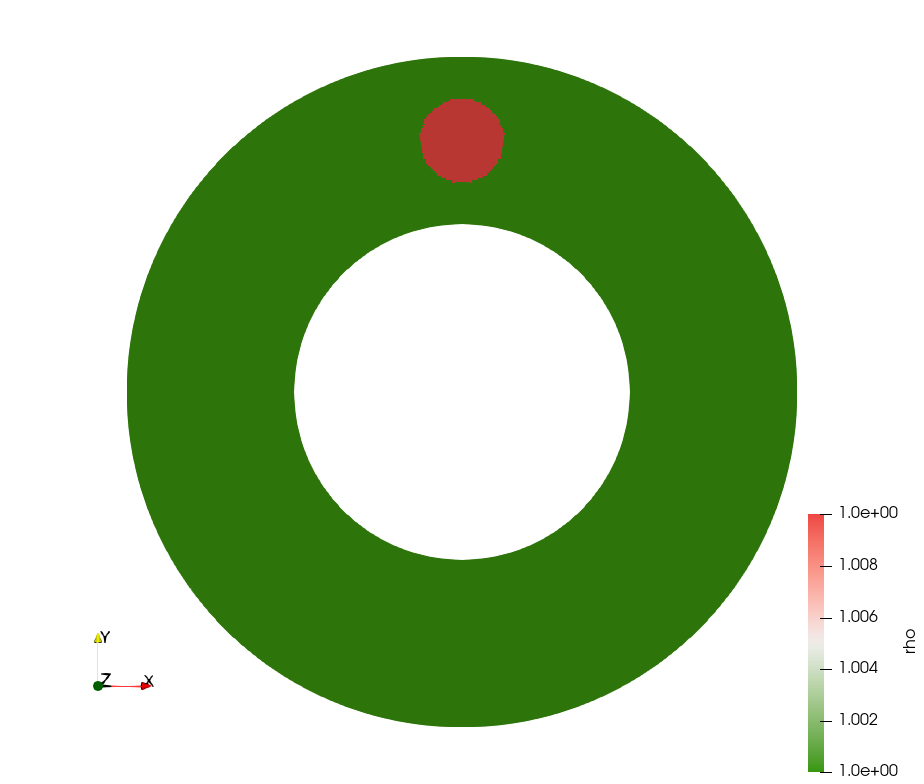
\includegraphics[width=5.6cm]{python_codes/fieldstone_151/results/test5/rho}
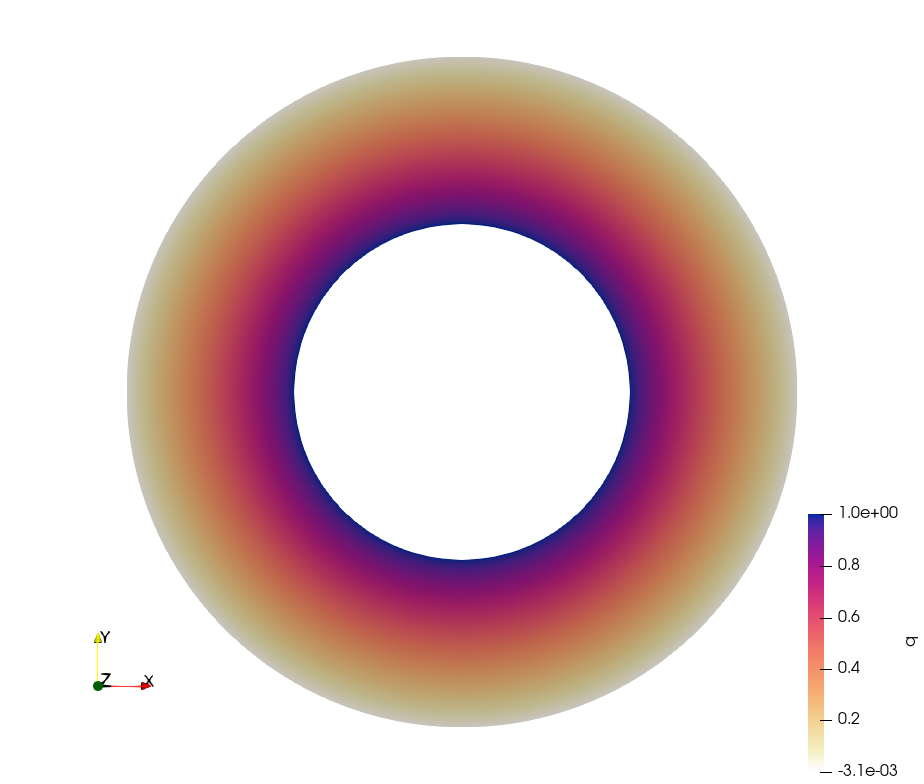
\includegraphics[width=5.6cm]{python_codes/fieldstone_151/results/test5/press}
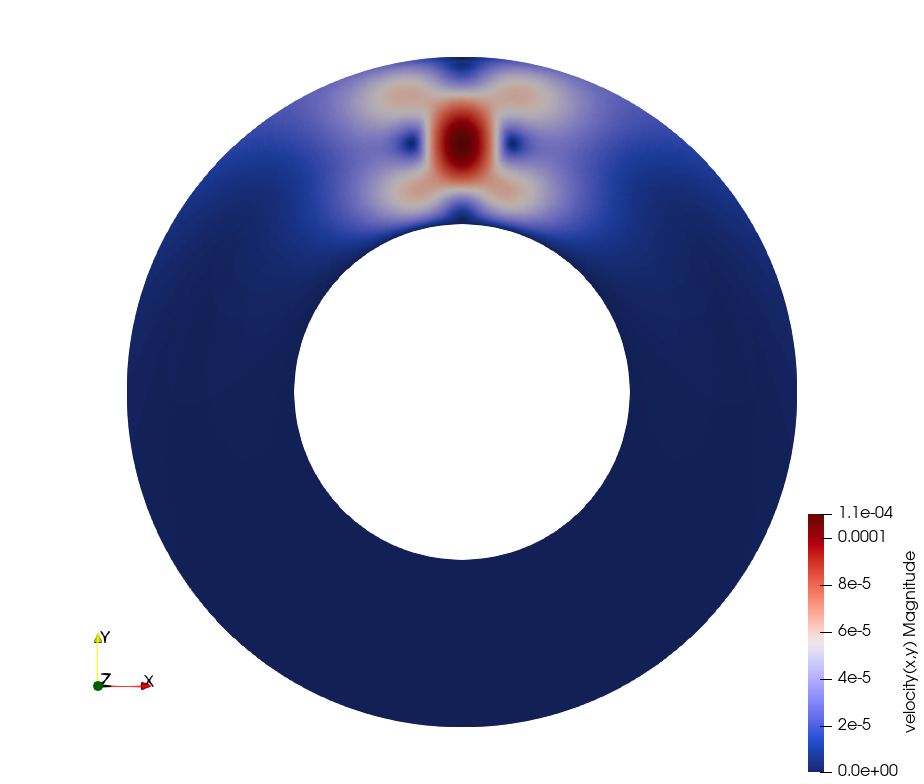
\includegraphics[width=5.6cm]{python_codes/fieldstone_151/results/test5/vel}\\
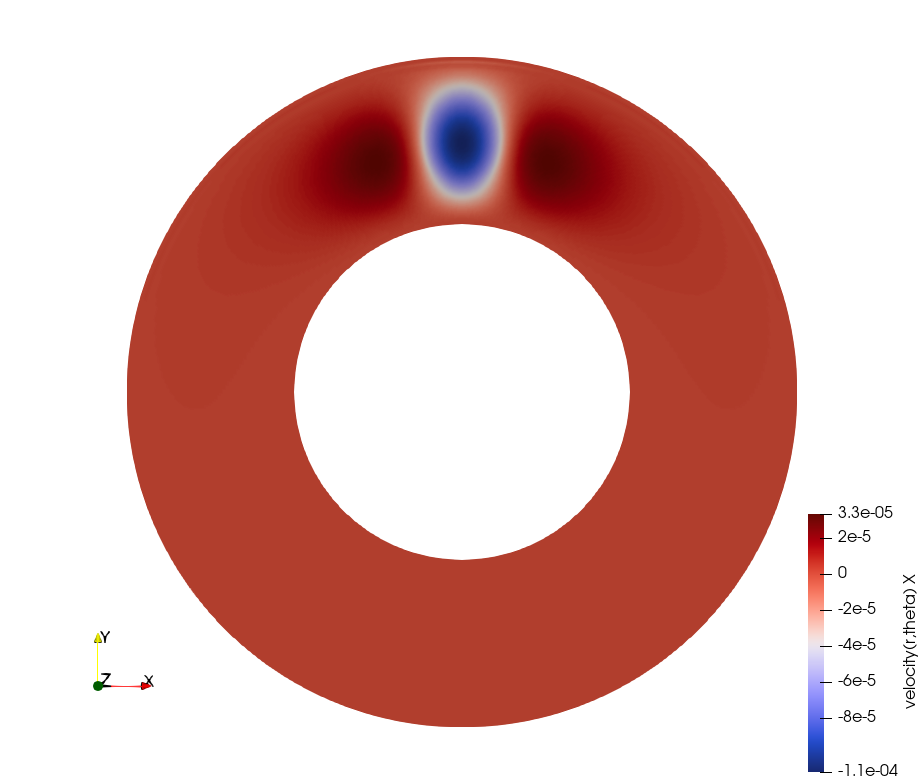
\includegraphics[width=5.6cm]{python_codes/fieldstone_151/results/test5/vr}
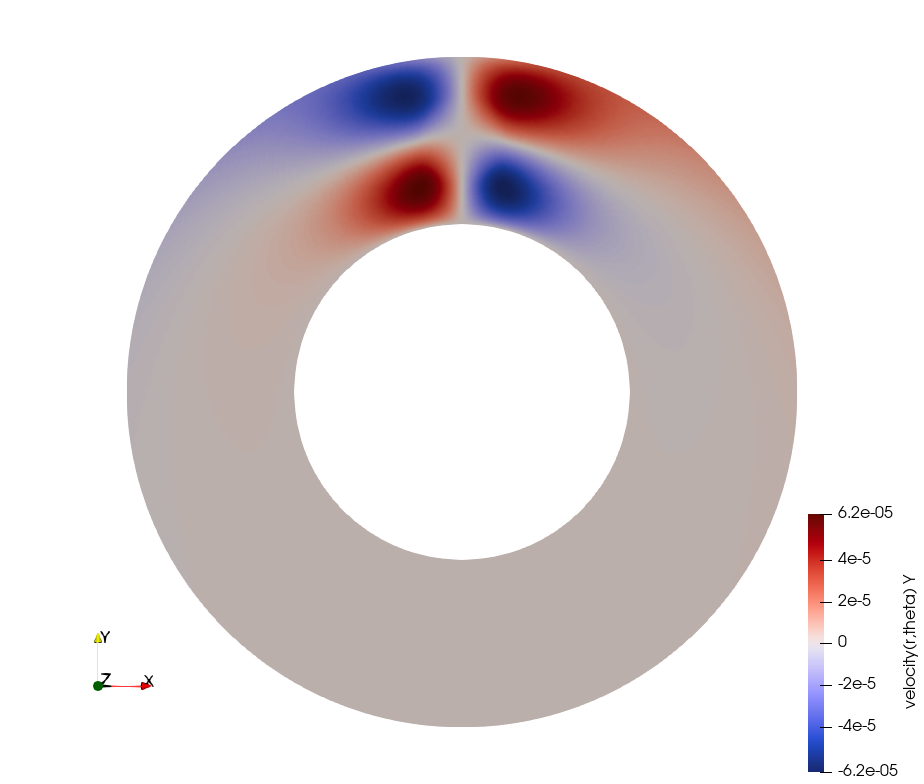
\includegraphics[width=5.6cm]{python_codes/fieldstone_151/results/test5/vt}
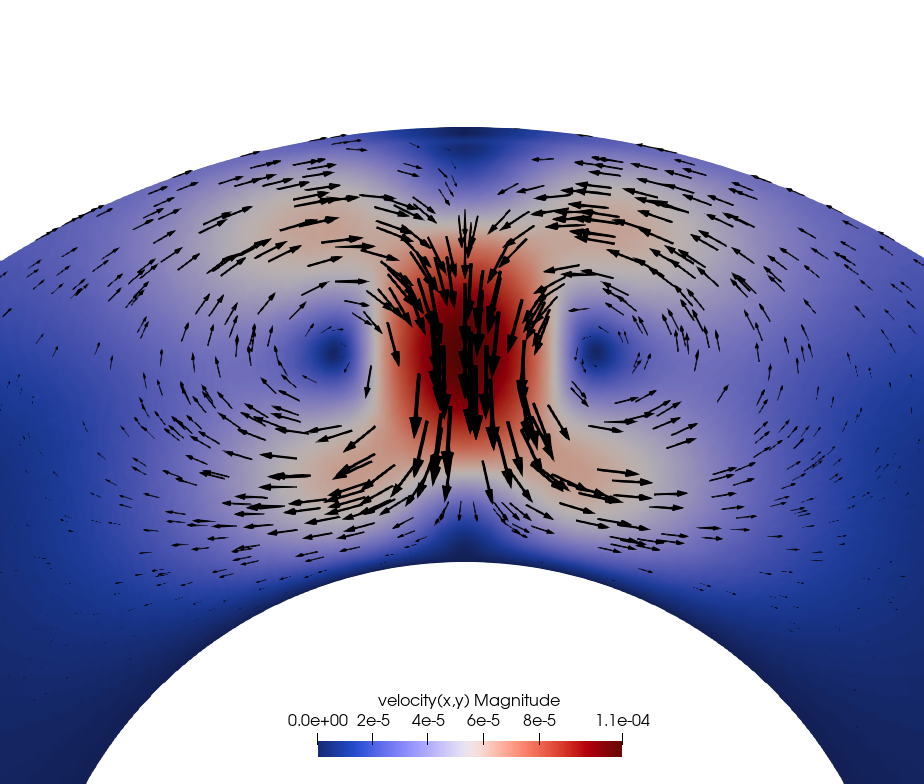
\includegraphics[width=5.6cm]{python_codes/fieldstone_151/results/test5/vel2}\\
{\captionfont resolution 32x384.}
\end{center}


\begin{center}
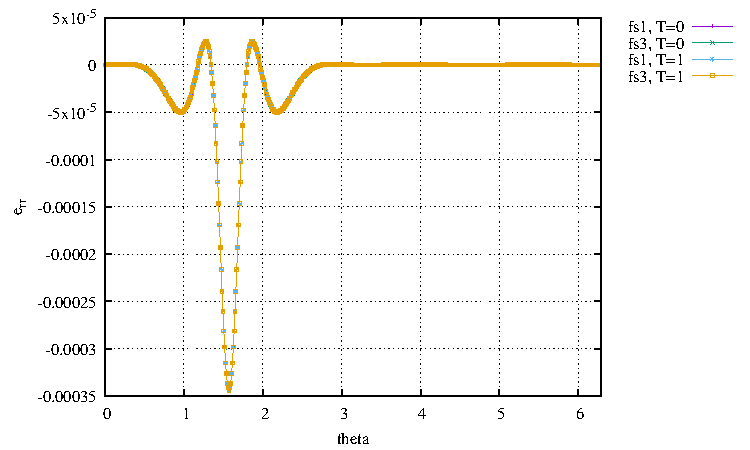
\includegraphics[width=8.5cm]{python_codes/fieldstone_151/results/test5/e_rr}
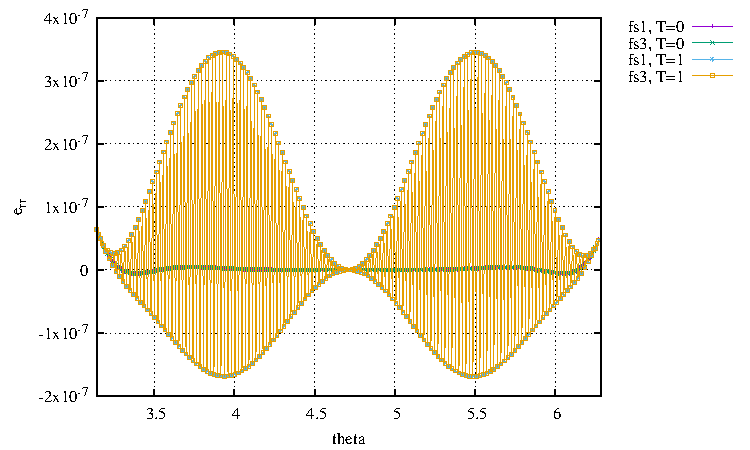
\includegraphics[width=8.5cm]{python_codes/fieldstone_151/results/test5/e_rr2}\\
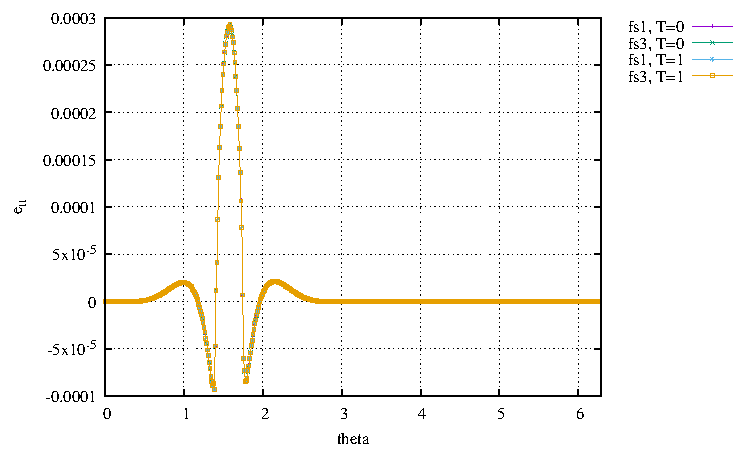
\includegraphics[width=8.5cm]{python_codes/fieldstone_151/results/test5/e_tt}
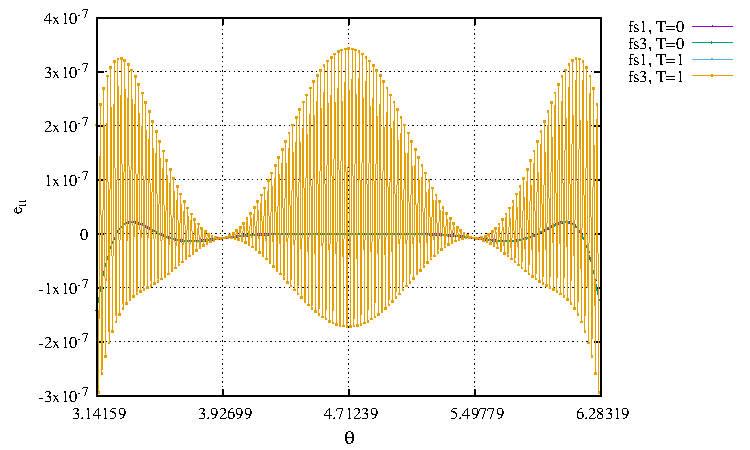
\includegraphics[width=8.5cm]{python_codes/fieldstone_151/results/test5/e_tt2}\\
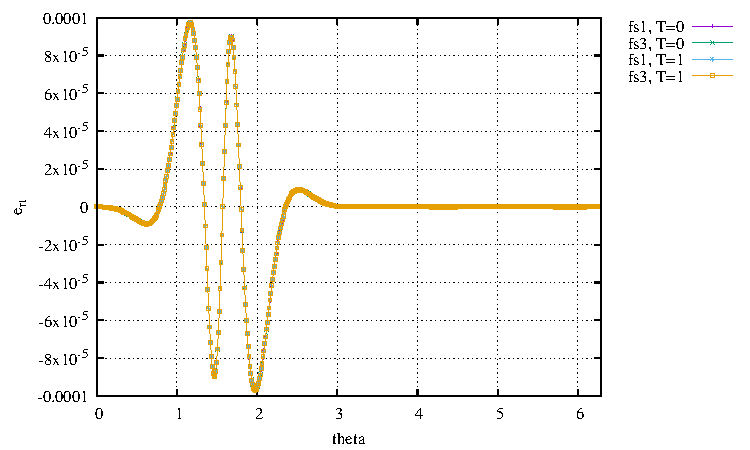
\includegraphics[width=8.5cm]{python_codes/fieldstone_151/results/test5/e_rt}
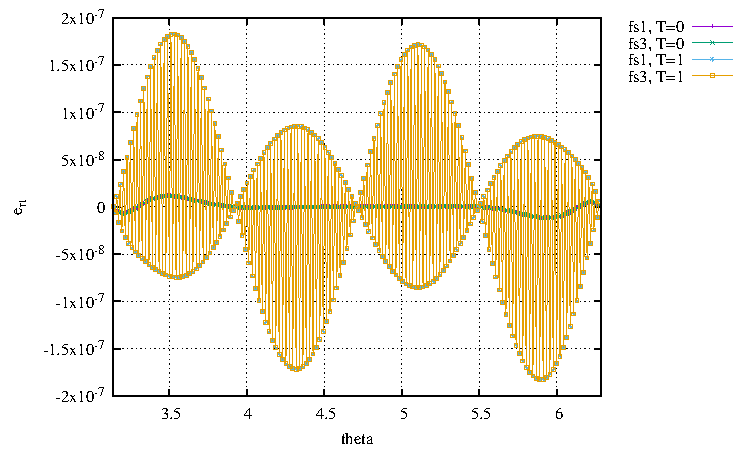
\includegraphics[width=8.5cm]{python_codes/fieldstone_151/results/test5/e_rt2}\\
{\captionfont Strain rate components at the surface, resolution 24x288. 
The first column of plots is the strain rate components all around the annulus at the surface, i.e.
$\theta\in[0,2\pi]$. The second column is the same components but plotted for $\theta\in[\pi,2\pi]$.
Zoom in to better see the results. 'T' stands for the trapezes variable.}
\end{center}


\begin{center}
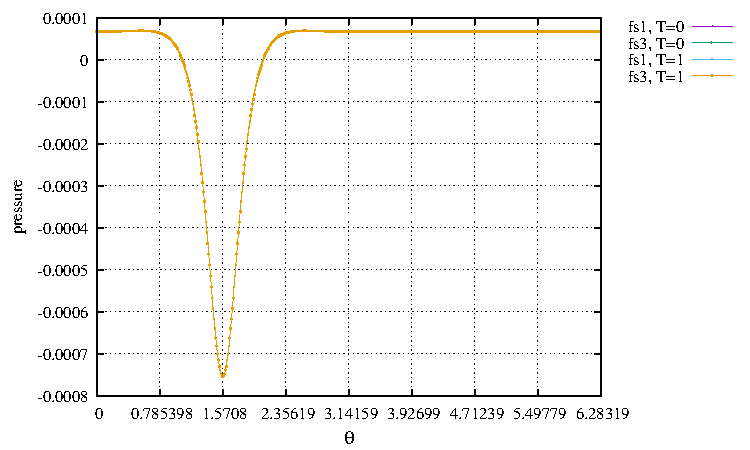
\includegraphics[width=8cm]{python_codes/fieldstone_151/results/test5/p}
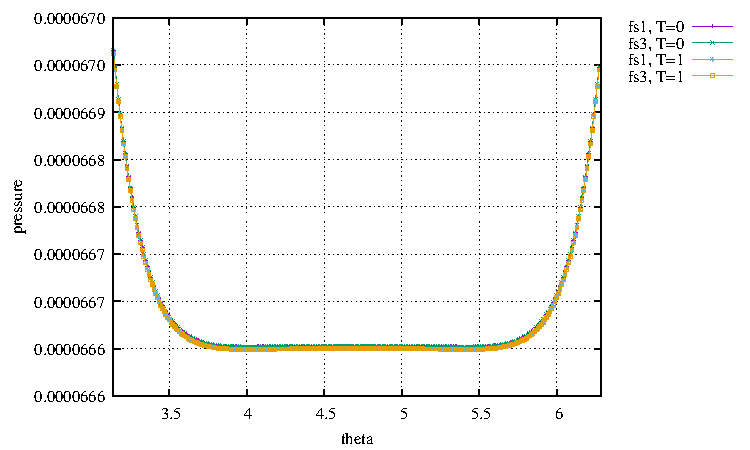
\includegraphics[width=8cm]{python_codes/fieldstone_151/results/test5/p2}\\
{\captionfont Pressure at the surface, resolution 24x288.}
\end{center}

%%%%%%%%%%%%%%%%%%%%%%%%%%%%%%%%%%%%%%%%%
\subsection*{test \#6: aquarium - free slip}

This test is inspired by \textcite{behr04}. Results obtained with {\tt script6}.
Density is constant, viscosity is constant, but now gravity is given by $\vec{g}=(0,-g_0)$.
Free slip boundary conditions are used. We expect zero flow and yet ...


\begin{center}
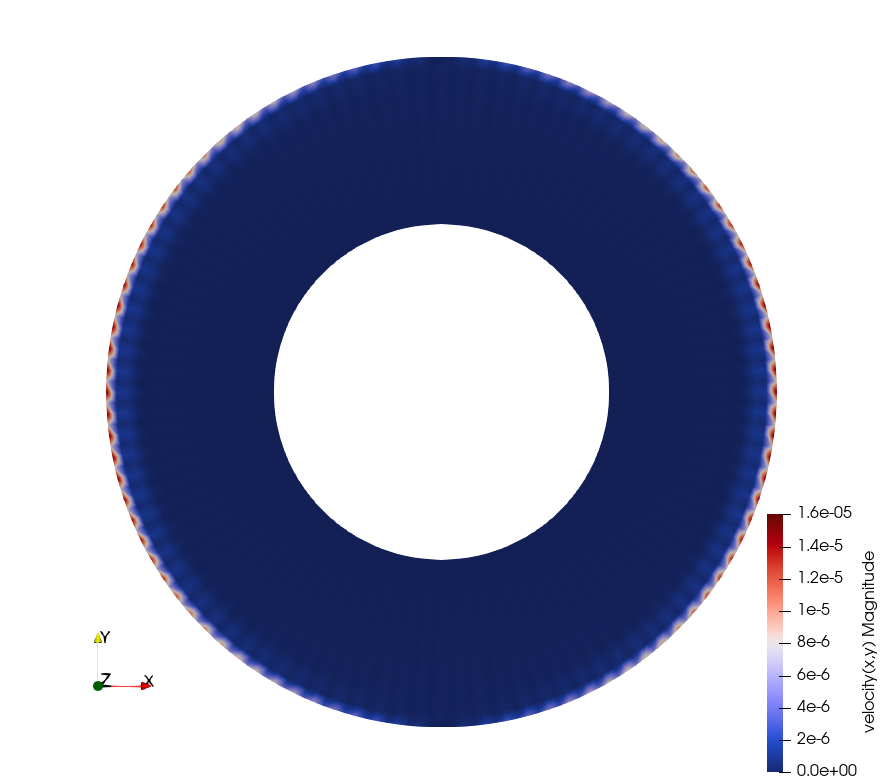
\includegraphics[width=8cm]{python_codes/fieldstone_151/results/test6/vel}
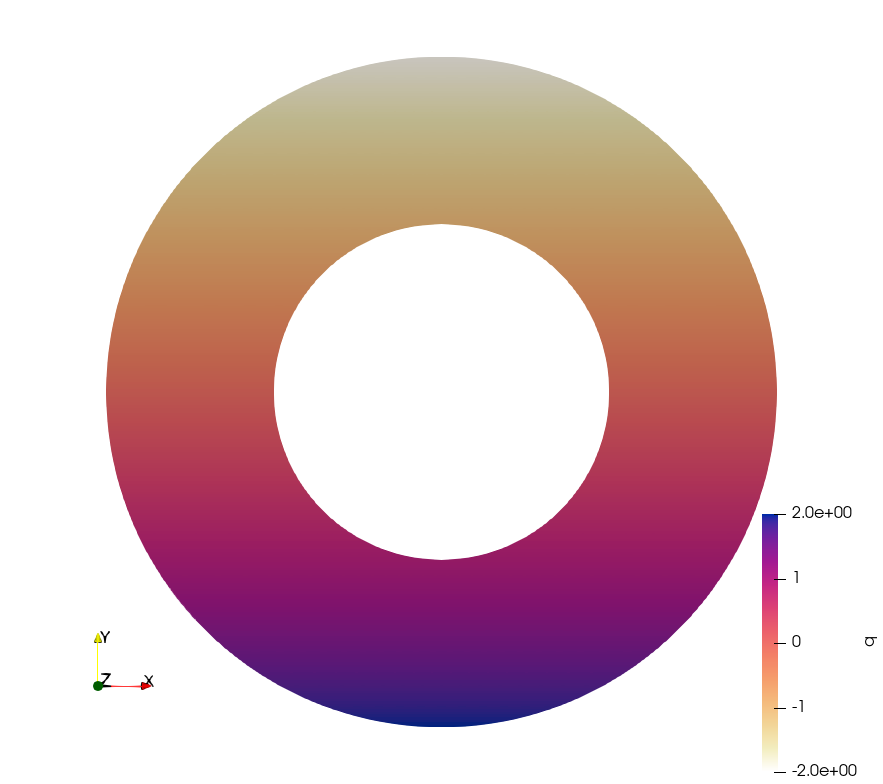
\includegraphics[width=8cm]{python_codes/fieldstone_151/results/test6/press}\\
{\captionfont Velocity and pressure fields, resolution $8\times 96$.}
\end{center}

The analytical solution is $\vec\upnu=(0,0)$ and $p(x,y)=-R_2+i\rho_0 g_0(R_2-y)$ so 
we can compute the velocity and pressure errors as a function of the mesh size $h$:

\begin{center}
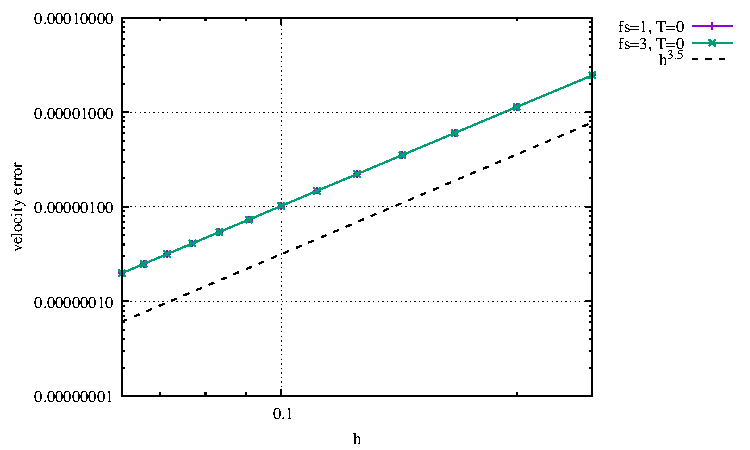
\includegraphics[width=8cm]{python_codes/fieldstone_151/results/test6/errv}
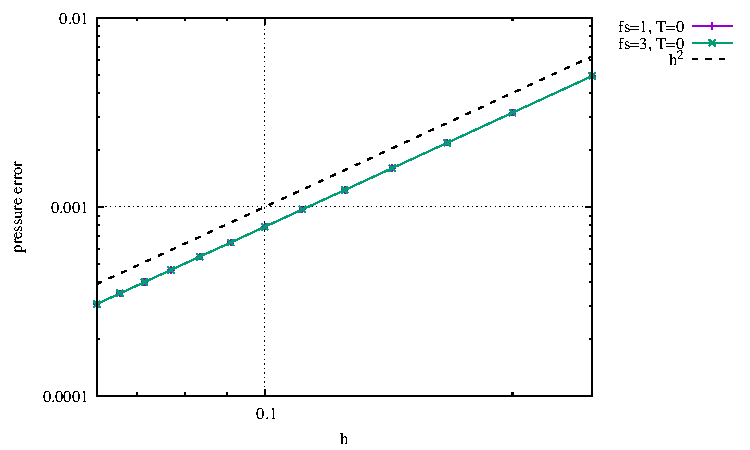
\includegraphics[width=8cm]{python_codes/fieldstone_151/results/test6/errp}
\end{center}





%%%%%%%%%%%%%%%%%%%%%%%%%%%%%%%%%%%%%%%%%%%%%%%%%%%%%%%%%%%%%%%%%%%%%%%%%%%%%%%%%%%%%%%%%%%%%%%%%%%
\subsection*{Conclusions}

The conclusion is unescapable: either way of prescribing free slip is fine, they yield 
virtuallly identical results. The trapeze option should not be used.  


%%%%%%%%%%%%%%%%%%%%%%%%%%%%%%%%%%%%%%%%%%%%%%%%%%%%%%%%%%%%%%%%%%%%%%%%%%%%%%%%%%%%%%%%%%%%%%%%%%%
\par\noindent\rule{\textwidth}{0.4pt}

\vspace{.5cm}

\begin{center}
\fbox{\begin{minipage}{0.9\textwidth}
{\color{teal}To Do, open questions, future work?}
\begin{itemize}
\item analytical solution test 3 ?
\item design more appropriate flow solution and test 3 methods to compute strain rate
\item implement axisymmetric calculations
\item check \fullcite{ensg82}
\item make sure that conversion between cartesian strain rate and cylindrical strain rate is correct
\item from my experience with stone 152, it is not clear how the additional terms in the matrix
wrt Lagrange multipliers should be scaled
\item check \fullcite{siwi20}
\item check \fullcite{urgf14}
\item check \fullcite{diur15}
\item check \fullcite{layt99}
\end{itemize}
\end{minipage}}
\end{center}

\newpage

Following \textcite{diur15} we add the following term to the weak form 
of the momentum equation:
\[
\int_\Gamma \vec{u}\cdot \vec{n} \; \vec{v}  \cdot \vec{n} d\Gamma  \qquad \forall \vec{v}
\]
where $\epsilon >0$ has a small value destined to converge to 0 and 
$\Gamma$ is the portion of the boundary where slip boundary conditions are to 
be implemented.
We have
\begin{eqnarray}
\vec{u}\cdot \vec{n} \quad \vec{v}  \cdot \vec{n} 
&=& (u_x n_x + u_y n_y) (v_x n_x+v_y n_y)  \\
&=& u_xv_x n_x^2 + u_y v_y n_y^2 + (u_xv_y +u_yv_x) n_x n_y  \\
&=& v_x(n_x^2 u_x + n_xn_y u_y) + v_y (n_xn_y u_x + n_y^2 u_y) \\
&=& (v_x \; v_y) \cdot
\left(
\begin{array}{c}
n_x^2 u_x + n_xn_y u_y\\
n_xn_y u_x + n_y^2 u_y
\end{array}
\right) \\
&=& 
(v_x \; v_y)
\cdot
\left(
\begin{array}{cc}
n_x^2 & n_xn_y \\
n_xn_y & n_y^2
\end{array}
\right)
\cdot
\left(
\begin{array}{c}
u_x \\ u_y
\end{array}
\right)\\
&=& 
(v_x \; v_y)
\cdot
\left(
\begin{array}{cc}
n_x^2 & n_xn_y \\
n_xn_y & n_y^2
\end{array}
\right)
\cdot
\left(
\begin{array}{c}
\sum_i \bN_i u_{x,i} \\ \sum _i \bN_i u_{y,i}
\end{array}
\right)\\
\end{eqnarray}










